\documentclass{standalone}
\usepackage{tikz}
\usetikzlibrary{decorations.pathreplacing}

\begin{document}

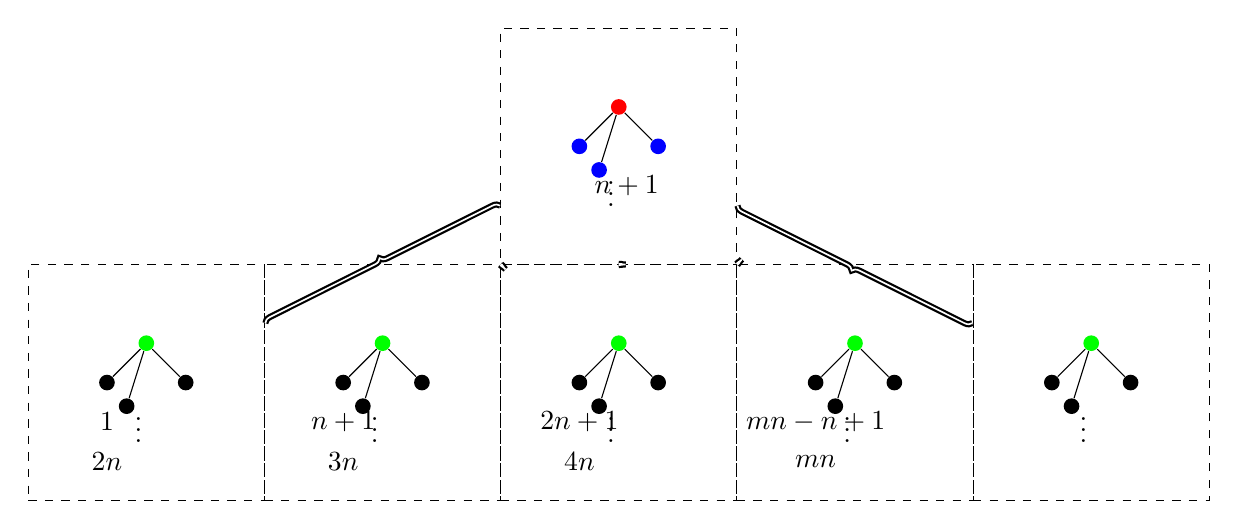
\begin{tikzpicture}
    % Colors
    \def\redcolor{red}
    \def\bluecolor{blue}
    \def\greencolor{green}
    \def\blackcolor{black}

    % First row - top
    \node[draw, dashed, inner sep=5pt, minimum size=3cm] (top) at (0, 3) {};
    \node[circle, fill=\redcolor, inner sep=2pt] (top-center) at (0, 3.5) {};
    \node[circle, fill=\bluecolor, inner sep=2pt] (top-left) at (-0.5, 3) {};
    \node[circle, fill=\bluecolor, inner sep=2pt] (top-left-2) at (-0.25, 2.7) {};
    \node[draw=none] at (-0.1, 2.5) {$\vdots$};
    \node[circle, fill=\bluecolor, inner sep=2pt] (top-right) at (0.5, 3) {};
    \node[draw=none] at (0.1, 2.5) {$n+1$};

    % Connections in top row
    \draw (top-center) -- (top-left);
    \draw (top-center) -- (top-left-2);
    \draw (top-center) -- (top-right);

    % Second row - bottom
    \foreach \i in {1, 2, 3, 4, 5} {
        \node[draw, dashed, inner sep=5pt, minimum size=3cm] (bot\i) at ({(\i-3)*3}, 0) {};
        \node[circle, fill=\greencolor, inner sep=2pt] (bot\i-center) at ({(\i-3)*3}, 0.5) {};
        \node[circle, fill=\blackcolor, inner sep=2pt] (bot\i-left) at ({(\i-3)*3-0.5}, 0) {};
        \node[circle, fill=\blackcolor, inner sep=2pt] (bot\i-left-2) at ({(\i-3)*3-0.25}, -0.3) {};
        \node[draw=none] at ({(\i-3)*3-0.1}, -0.5) {$\vdots$};
        \node[circle, fill=\blackcolor, inner sep=2pt] (bot\i-right) at ({(\i-3)*3+0.5}, 0) {};
    }

    % Connections in bottom row
    \foreach \i in {1, 2, 3, 4, 5} {
        \draw (bot\i-center) -- (bot\i-left);
        \draw (bot\i-center) -- (bot\i-left-2);
        \draw (bot\i-center) -- (bot\i-right);
    }

    % Labels for bottom row
    \node[draw=none] at (-6.5, -0.5) {1};
    \node[draw=none] at (-6.5, -1) {$2n$};

    \node[draw=none] at (-3.5, -0.5) {$n+1$};
    \node[draw=none] at (-3.5, -1) {$3n$};

    \node[draw=none] at (-0.5, -0.5) {$2n+1$};
    \node[draw=none] at (-0.5, -1) {$4n$};

    \node[draw=none] at (2.5, -0.5) {$mn-n+1$};
    \node[draw=none] at (2.5, -1) {$mn$};

    % Double lines between top and bottom row
    \draw[thick, double, decoration={brace, mirror}, decorate] (top) -- (bot1);
    \draw[thick, double, decoration={brace, mirror}, decorate] (top) -- (bot2);
    \draw[thick, double, decoration={brace, mirror}, decorate] (top) -- (bot3);
    \draw[thick, double, decoration={brace, mirror}, decorate] (top) -- (bot4);
    \draw[thick, double, decoration={brace, mirror}, decorate] (top) -- (bot5);

\end{tikzpicture}

\end{document}